\documentclass{article} 
\usepackage{polski} 
\usepackage[utf8]{inputenc} 
\usepackage[OT4]{fontenc} 
\usepackage{graphicx,color} 
\usepackage{url}
\usepackage{float}
\usepackage[pdftex,hyperfootnotes=false,pdfborder={0 0 0}]{hyperref} %za wszystkimi pakietami; pdfborder nie wszedzie tak samo zaimplementowane bo specyfikacja nieprecyzyjna; pod miktex'em po prostu nie widac wtedy ramek

% Zmiana rozmiarów strony tekstu
\addtolength{\voffset}{-1cm}
\addtolength{\hoffset}{-1cm}
\addtolength{\textwidth}{2cm}
\addtolength{\textheight}{2cm}

%bardziej zyciowe parametry sterujace rozmieszczeniem rysunkow
\renewcommand{\topfraction}{.85}
\renewcommand{\bottomfraction}{.7}
\renewcommand{\textfraction}{.15}
\renewcommand{\floatpagefraction}{.66}
\renewcommand{\dbltopfraction}{.66}
\renewcommand{\dblfloatpagefraction}{.66}
\setcounter{topnumber}{9}
\setcounter{bottomnumber}{9}
\setcounter{totalnumber}{20}
\setcounter{dbltopnumber}{9}

% własny bullet list z malymi odstepami
\newenvironment{tightlist}{
\begin{itemize}
  \setlength{\itemsep}{1pt}
  \setlength{\parskip}{0pt}
  \setlength{\parsep}{0pt}}
{\end{itemize}}

%obrazkow szukamy w nastepujacym katalogu:
\graphicspath{{pics/}}



%\title{Sprawozdanie z laboratorium:\\Metaheurystyki i Obliczenia Inspirowane Biologicznie}
%\author{}
%\date{}


\begin{document}

\thispagestyle{empty} %bez numeru strony

\begin{center}
{\large{Sprawozdanie z laboratorium:\\
Uczenie Maszynowe i Sieci Neuronowe}}

\vspace{3ex}


\vspace{3ex}
{\footnotesize\today}

\end{center}


\vspace{10ex}

Prowadzący: dr hab.~inż. Maciej Komosiński

\vspace{5ex}

Autorzy:
\begin{tabular}{lllr}
\textbf{Maciej Trojan} & inf94378 & ISWD & maciek.trojan@me.com \\
\textbf{Paweł Rychły } & inf94362 & ISWD & pawelrychly@gmail.com \\
\end{tabular}

\vspace{5ex}

Zajęcia środowe, 11:45.


\newpage


\section{Uczenie nadzorowane sztucznych sieci neuronowych}

\paragraph{Zadanie 2. Różnice funkcjonalne pomiędzy sieciami jedno- i wielowarstwowymi oraz pomiędzy sieciami liniowymi a nieliniowymi (uczenie sieci warstwowych funkcji logicznej AND i funkcji różnicy symetrycznej XOR)}

\subparagraph{1. Skonstruuj zbiór przykładów definiujący dwuargumentową funkcję ("bramkę") AND (File|New|Data set) i zachowaj go. Wszystkie 4 przykłady mają stanowić zbiór uczący. Jakie są klasy decyzyjne w tym zbiorze przykładów i jakie są ich liczności?\\}

Zbiór zawiera dwie klasy decyzyjne: 1 i 0. Ich liczności wynoszą odpowiednio: 1 i 3. 

\begin{table}[h]
    \begin{tabular}{|c|c|c|}
     \hline
     	VAR1 & VAR2 & decyzja \\ \hline
        0 & 0 & 0 \\ 
        0 & 1 & 0 \\ 
		1 & 0 & 0 \\ 
		1 & 1 & 1 \\ \hline             
    \end{tabular}
    \caption{Zbiór przykładów uczących}
\end{table} 

\subparagraph{3. Wyobraź sobie (narysuj) pożądaną funkcję odpowiedzi sieci (trójwymiarowy wykres zależności wyjścia od dwóch wejść)\\}

\begin{figure}[H]
\begin{center}
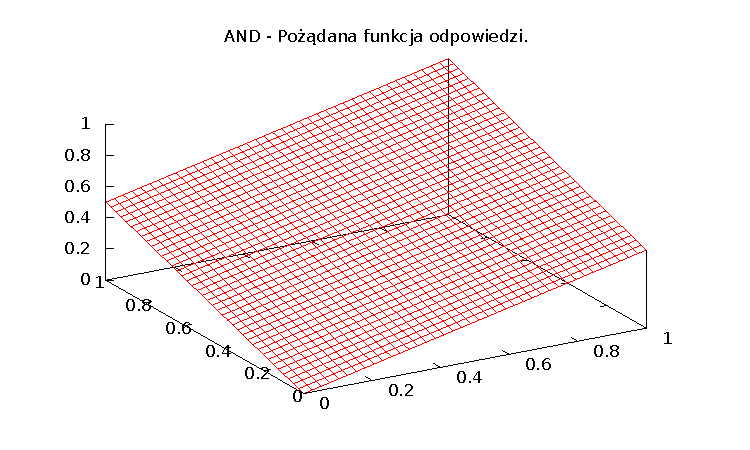
\includegraphics[width=1\textwidth]{pozodana_funnkcja_odpowiedzi_and.pdf}
\end{center}
\caption{Pożądana funkcja odpowiedzi sieci}
\label{fig-1Tdelta}
\end{figure}

\subparagraph{4. Skonstruuj liniową sieć jednowarstwową o architekturze 2-1 (File|New|Network, Type=Linear, przycisk Advise). Uaktywnij okno wykresu błędu średniokwadratowego (Statistics|Training graph). Naucz sieć na problemie AND (Train|Multilayer perceptron|Back propagation). Obejrzyj funkcję odpowiedzi sieci (Run|Responce surface) i błędy dla poszczególnych przypadków (Statistics|Case errors)\\}

\begin{figure}[H]
\begin{center}
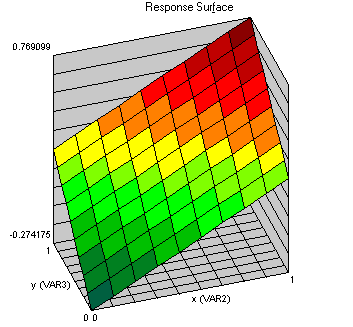
\includegraphics[width=0.5\textwidth]{And-training-3D.png}
\end{center}
\caption{Funkcja odpowiedzi sieci}
\label{fig-1Tdelta}
\end{figure}

\begin{figure}[H]
\begin{center}
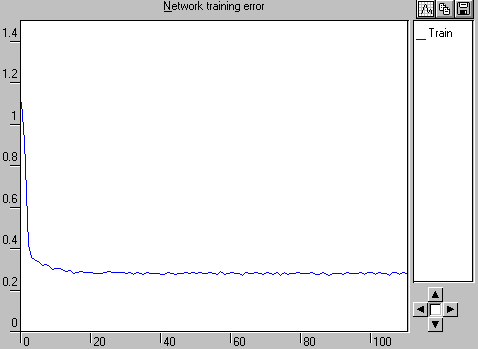
\includegraphics[width=0.5\textwidth]{And-training-Error.png}
\end{center}
\caption{Wykres błędu}
\label{fig-1Tdelta}
\end{figure}

\begin{figure}[H]
\begin{center}
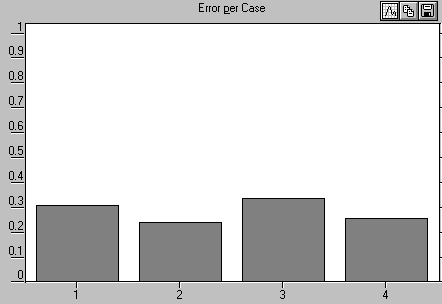
\includegraphics[width=0.5\textwidth]{And-training-CaseError.png}
\end{center}
\caption{Błędy dla poszczególnych przypadków}
\label{fig-1Tdelta}
\end{figure}
 
\subparagraph{5. Spróbuj utworzyć sieć liniową dla problemu AND o liczbie warstw większej niż 2.\\}
Program Statistica uniemożliwia utworzenie takiej sieci.

\subparagraph{6. Przerób sieć na nieliniową sieć jednowarstwową (ustawiając Act fn w Edit|Network na Logistic) i naucz ją na tym samym problemie.}

\begin{figure}[H]
\begin{center}
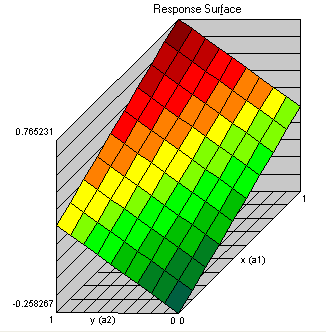
\includegraphics[width=0.5\textwidth]{And-training-3D-logistic.png}
\end{center}
\caption{Funkcja odpowiedzi sieci}
\label{fig-1Tdelta}
\end{figure}

\begin{figure}[H]
\begin{center}
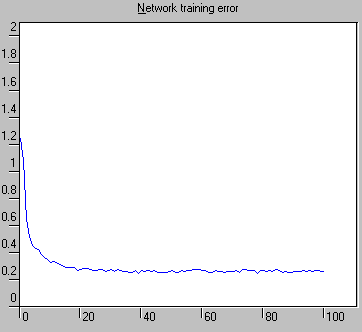
\includegraphics[width=0.5\textwidth]{And-training-Error-logistic.png}
\end{center}
\caption{Wykres błędu}
\label{fig-1Tdelta}
\end{figure}

\begin{figure}[H]
\begin{center}
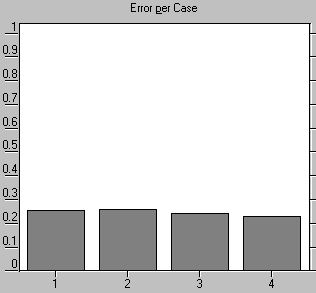
\includegraphics[width=0.5\textwidth]{And-training-CaseError-logistic.png}
\end{center}
\caption{Błędy dla poszczególnych przypadków}
\label{fig-1Tdelta}
\end{figure}

\subparagraph{7. Wejdź do edytora sieci (Network|Edit) i przypatrz się wagom neuronu wyjściowego. Wykreśl w przestrzeni wejść prostą, którą definiuje neuron wyjściowy i oceń, czy i jak realizuje ona separację klas decyzyjnych. \\}
wagi: \\
w0 = 0.2847 \\
w1 = 0.5152 \\
w2 = 0.4980 \\

\begin{figure}[H]
\begin{center}
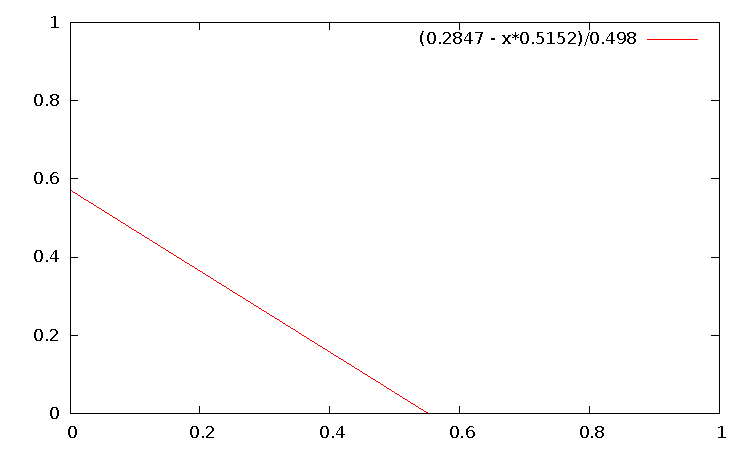
\includegraphics[width=0.75\textwidth]{and-prosta-wagi.pdf}
\end{center}
\caption{Prosta w przestrzeni wejść definiująca neuron wyjściowy}
\label{fig-1Tdelta}
\end{figure}

Prosta dokonuje niepoprawnej separacji klas decyzyjnych. Zgodnie z narysowaną prostą przypadki 0, 1 oraz 1, 0 należałyby do klasy 1.


\subparagraph{8. Skonstruuj zbiór przykładów definiujący dwuargumentową funkcję XOR i zachowaj go. Wszystkie 4 przykłady mają stanowić zbiór uczący. \\}

\begin{table}[h]
    \begin{tabular}{|c|c|c|}
     \hline
     	VAR1 & VAR2 & decyzja \\ \hline
        0 & 0 & 0 \\ 
        0 & 1 & 1 \\ 
		1 & 0 & 1 \\ 
		1 & 1 & 0 \\ \hline             
    \end{tabular}
    \caption{Zbiór przykładów uczących}
\end{table} 



\subparagraph{9. Wyobraź sobie (narysuj) pożądaną funkcję odpowiedzi sieci.\\}

\begin{figure}[H]
\begin{center}
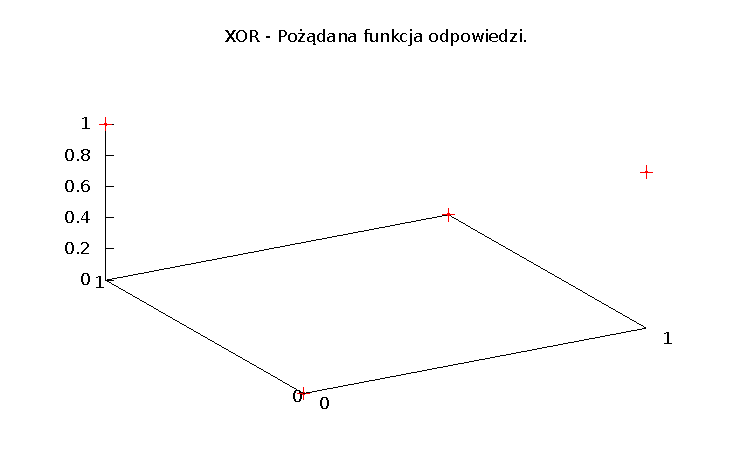
\includegraphics[width=1\textwidth]{pozodana_funnkcja_odpowiedzi_xor.pdf}
\end{center}
\caption{Pożądana funkcja odpowiedzi sieci}
\label{fig-1Tdelta}
\end{figure}

\subparagraph{10. Skonstruuj liniową sieć jednowarstwową o architekturze 2-1 i naucz ją na problemie XOR. Obejrzyj funkcję odpowiedzi sieci i błędy dla poszczególnych przypadków.\\}

\begin{figure}[H]
\begin{center}
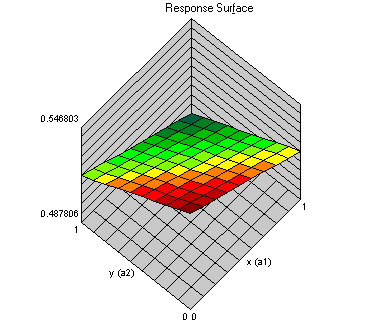
\includegraphics[width=0.5\textwidth]{Xor-training-3D.png}
\end{center}
\caption{Funkcja odpowiedzi sieci}
\label{fig-1Tdelta}
\end{figure}

\begin{figure}[H]
\begin{center}
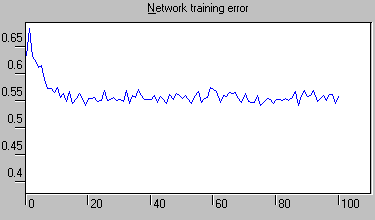
\includegraphics[width=0.5\textwidth]{Xor-training-Error.png}
\end{center}
\caption{Wykres błędu}
\label{fig-1Tdelta}
\end{figure}

\begin{figure}[H]
\begin{center}
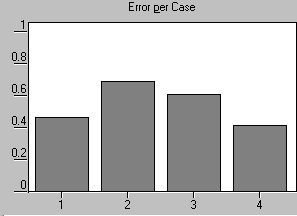
\includegraphics[width=0.5\textwidth]{Xor-training-CaseError.png}
\end{center}
\caption{Błędy dla poszczególnych przypadków}
\label{fig-1Tdelta}
\end{figure}
 
\subparagraph{11. Przerób sieć na nieliniową sieć jednowarstwową i naucz ją na tym samym problemie (zwróć uwagę, jak sieć stara się minimalizować błąd). Obejrzyj, jak zmienia się rozkład wag podczas procesu uczenia (Statistics|Weight distribution).\\}

\begin{figure}[H]
\begin{center}
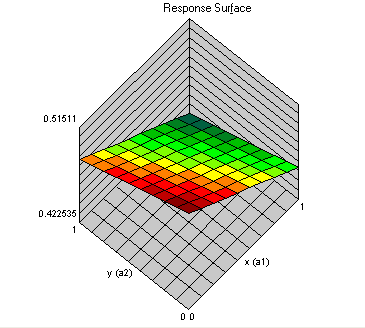
\includegraphics[width=0.5\textwidth]{Xor-training-3D-logistic.png}
\end{center}
\caption{Funkcja odpowiedzi sieci}
\label{fig-1Tdelta}
\end{figure}

\begin{figure}[H]
\begin{center}
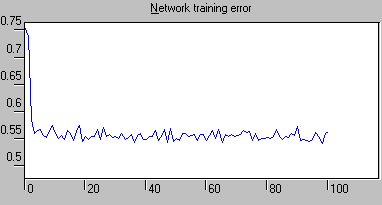
\includegraphics[width=0.5\textwidth]{Xor-training-Error-logistic.png}
\end{center}
\caption{Wykres błędu}
\label{fig-1Tdelta}
\end{figure}

\begin{figure}[H]
\begin{center}
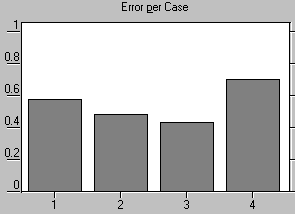
\includegraphics[width=0.5\textwidth]{Xor-training-CaseError-logistic.png}
\end{center}
\caption{Błędy dla poszczególnych przypadków}
\label{fig-1Tdelta}
\end{figure}

W trakcie procesu uczenia wartości wag zbiegały się do siebie. 

\subparagraph{12. Skonstruuj nieliniową sieć dwuwarstwową o architekturze 2-2-1 (File|New|Network, Type=Multilayer perceptron) i naucz ją na problemie XOR. Obejrzyj funkcję odpowiedzi.\\}

\begin{figure}[H]
\begin{center}
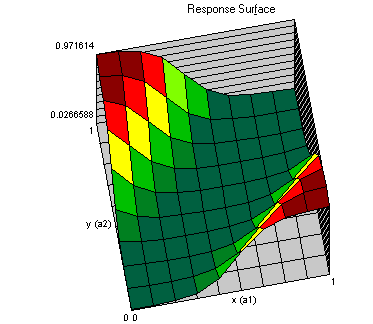
\includegraphics[width=0.5\textwidth]{Xor-multi-training-3D.png}
\end{center}
\caption{Funkcja odpowiedzi sieci}
\label{fig-1Tdelta}
\end{figure}

\begin{figure}[H]
\begin{center}
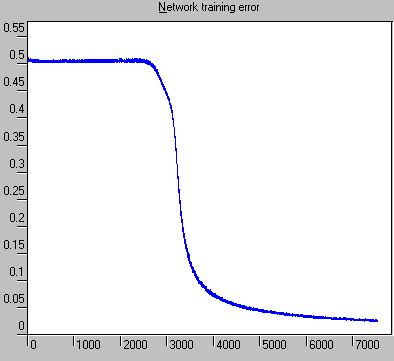
\includegraphics[width=0.5\textwidth]{Xor-multi-training-Error.png}
\end{center}
\caption{Wykres błędu}
\label{fig-1Tdelta}
\end{figure}

\begin{figure}[H]
\begin{center}
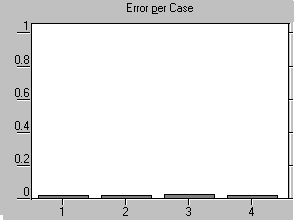
\includegraphics[width=0.5\textwidth]{Xor-multi-training-CaseError.png}
\end{center}
\caption{Błędy dla poszczególnych przypadków}
\label{fig-1Tdelta}
\end{figure}

\subparagraph{13. Obejrzyj wagi sieci w edytorze sieci (Edit|Network). Jakie proste definiują neurony w warstwie ukrytej (spróbuj je narysować w przestrzeni wejść) ? Jak można interpretować działanie neuronu wyjściowego ?\\}
\begin{table}[h]
    \begin{tabular}{|c|c|c|}
     \hline
        0 & h1\#01 &	h1\#02 \\ \hline 
        Th & -3.132	& 2.722 \\ 
		a1 & -6.088	& -5.279 \\ 
		a2 & 6.116 & 5.042 \\ \hline             
    \end{tabular}
    \caption{Wagi neuronów w warstwie ukrytej}
\end{table} 

\begin{figure}[H]
\begin{center}
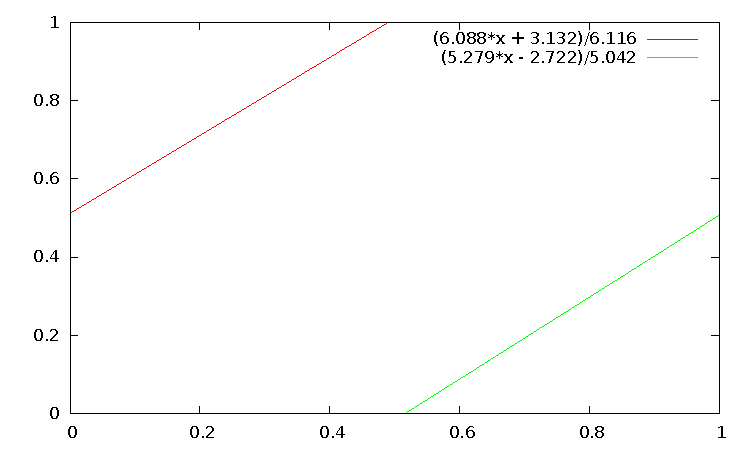
\includegraphics[width=0.75\textwidth]{xor-multi-prosta-wagi.pdf}
\end{center}
\caption{Proste wyznaczone przez neurony warstwy ukrytej}
\label{fig-1Tdelta}
\end{figure}
Neuron wyjściowy agreguje informacje pochodzące z neuronów ukrytych. Wagi neuronów warstw ukrytych definiują płaszczyzny w przestrzeni wejść. Neuron wyjściowy dokonuje klasyfikacji, w oparciu o te płaszczyzny.   

\subparagraph{14. Obejrzyj, jak zmienia się rozkład wag podczas procesu uczenia. Jaka jest przyczyna takiego zachowania wag i jakie to może mieć konsekwencje (z "informatycznego" punktu widzenia) ?\\}

W trakcie uczenia sieci, wartości bezwzględne wag systematycznie rosną. Może to doprowadzić do przekroczenia zakresu liczb.

\paragraph{Zadanie 3. Obserwacja zjawiska przeuczenia na przykładzie zbioru PIMA}
\subparagraph{2. Wczytaj zbiór PIMA i skonstruuj dla niego dwuwarstwową sieć nieliniową o architekturze 8-4-1.\\}
\begin{figure}[H]
\begin{center}
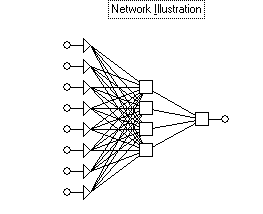
\includegraphics[width=0.5\textwidth]{8-4-1-zad3.png}
\end{center}
\caption{Dwuwarstwowa sieć neuronowa o architekturze 8-4-1.}
\label{fig-1Tdelta}
\end{figure}


\subparagraph{3. Obejrzyj ustawienia w okienku Pre/Post Processing.\\}

\begin{figure}[H]
\begin{center}
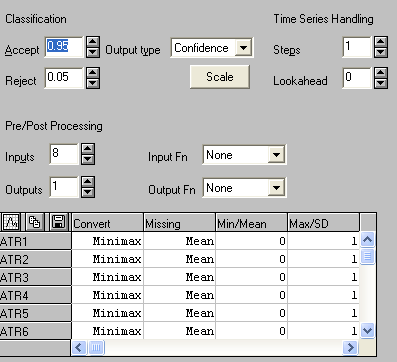
\includegraphics[width=0.5\textwidth]{8-4-1-zad3-pre-post-processing.png}
\end{center}
\caption{Okno Pre/Post Processing}
\label{fig-1Tdelta}
\end{figure}


\subparagraph{5. Przeprowadź uczenie algorytmem wstecznej propagacji błędu (może być bardzo długie, np. 20 000 epok); obserwuj przebieg błędu dla zbioru uczącego i weryfikującego.\\}

\begin{figure}[H]
\begin{center}
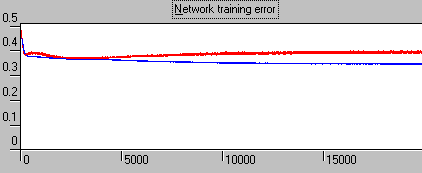
\includegraphics[width=0.5\textwidth]{8-4-1-zad3-przeuczenie.png}
\end{center}
\caption{Przebieg błędu dla zbioru uczącego i weryfikującego}
\label{fig-1Tdelta}
\end{figure}
Jak można zauważyć na powyższym wykresie, po około 5000 epok błąd średniokwadratowy dla zbioru weryfikującego zaczął rosnąć. Spowodowane jest to efektem przeuczenia.  

\paragraph{Zadanie 4. Dobór liczby neuronów w warstwie ukrytej na przykładzie zbioru IRIS.}
\subparagraph{3. Czy istnieje jednoznaczna zależność pomiędzy n a przebiegiem błędu średniokwadratowego? Czy biorąc pod uwagę tylko przebeg błędu dla zbioru uczącego można ustalić optymalną liczbę neuronów w warstwie ukrytej? Jeśli tak, to ile ona wynosi dla tego zbioru przykładów?}

\begin{figure}[H]
\begin{center}
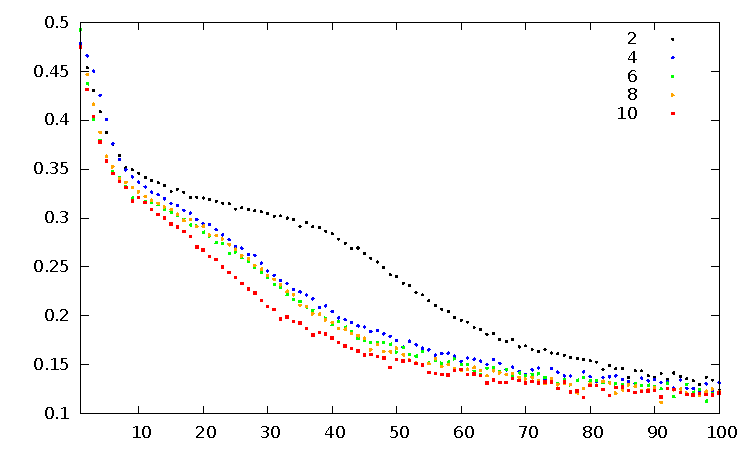
\includegraphics[width=1\textwidth]{zad_4_blad_n.pdf}
\end{center}
\caption{Przebieg błędu uczenia w zależności od liczby neuronów w warstwie ukrytej}
\label{fig-1Tdelta}
\end{figure}

Jak można zauważyć na powyższym wykresie, większa liczba neuronów w warstwie ukrytej spowodowała, że błąd w początkowych epokach uczenia spadał szybciej. Różnica ta malała jednak w kolejnych etapach. Nie można ustalić optymalnej liczby neuronów w warstwie ukrytej. 


\end{document}

